\section{System Overview and Preliminaries}
\label{sec:system}
\textsc{Synopsis} is a distributed sketch constructed over voluminous spatiotemporal data streams.
The number of sketchlets (executing on different machines) that comprise the distributed sketch varies dynamically as the system scales in or out to cope with data arrival rates and memory pressure.
%Each sketchlet is responsible for one or more geographical scopes and is implemented as a stateful stream processing node that can build and retain state over time.
A stream partitioning scheme, based on the Geohash algorithm (described below), is used to route packets to the appropriate sketchlet.
Sketchlets ingest stream packets and construct compact, in-memory representations of the observational data by extracting metadata from stream packets.
During dynamic scaling operations, the geographical extents managed by a sketch varies.
\vspace{1.5em} \\
\textbf{Geohash Algorithm} \\
We use the Geohash~algorithm~\cite{geohash} to balance load and partition incoming data streams across processing resources. Geohash divides the earth into a hierarchy of bounding boxes identified by Base 32 strings; the longer the geohash string, the more precise the bounding box. Figure~\ref{fig:geohash} illustrates this hierarchy. Most of the eastern United States is contained within the bounding box described by geohash \emph{D}, while \emph{DJ} encompasses substantial parts of Florida, Georgia, and Alabama. The bounding box \emph{DJKJ} (highlighted in red) contains Tallahassee, Florida. This hierarchical representation enables \textsc{Synopsis} to cope with both low- and high-density regions: several resources may be tasked with managing streams originating in and around large cities, while rural areas fall under the purview of a single node.

\begin{figure}[b!]
    \centerline{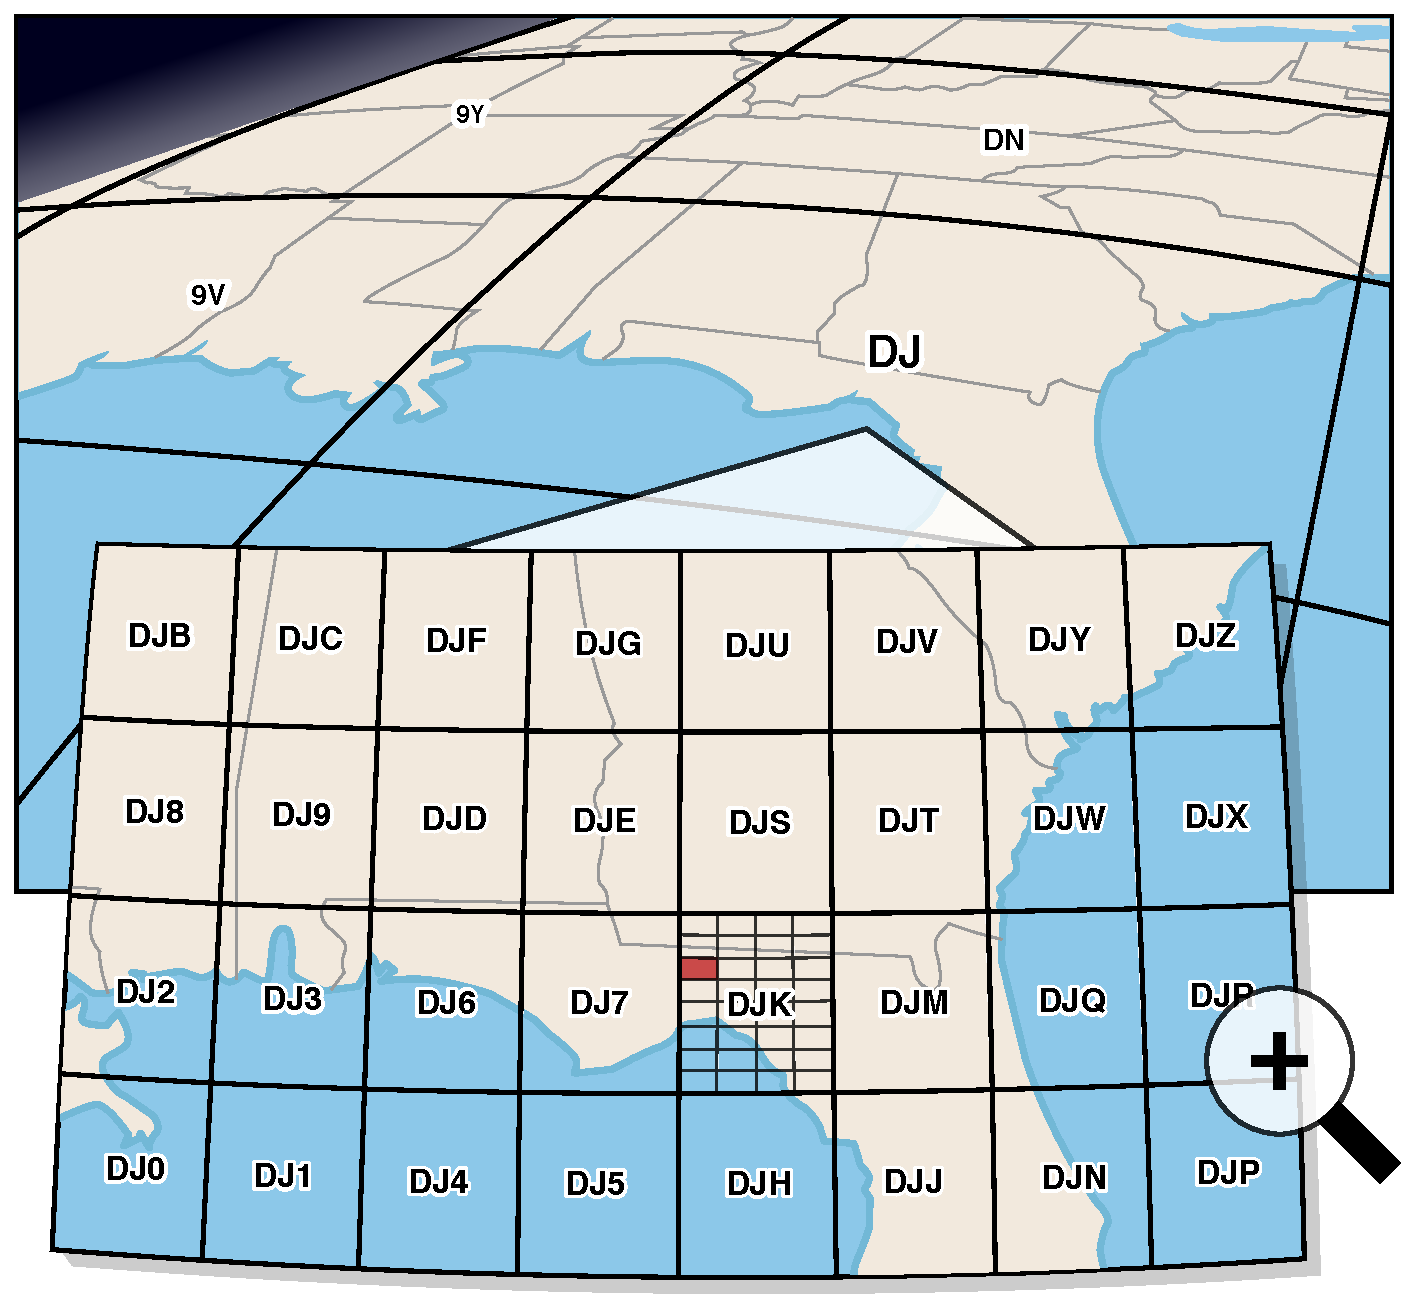
\includegraphics[width=2.75in]{figures/geohash.pdf}}
    \caption{A demonstration of the Geohash algorithm. Each additional character in a geohash describes a finer-grained region; geohash \emph{DJ} contains substantial parts of Florida, Georgia, and Alabama, USA, while \emph{DJKJ} (highlighted in red) encompasses Tallahassee.}
    \label{fig:geohash}
\end{figure}

To achieve fine-grained control over our geohash partitions, we operate at the bit level rather than Base 32 character level when routing streams. Each bit added to a geohash string reduces its scope by half, with each character represented by five bits ($2^5 = 32$). In other words, a four-character geohash string represents 20 spatial subdivisions applied recursively to each resulting region. This property allows us to manage and allocate resources across a wide variety of observational densities.

\textsc{Synopsis} relies on a set of auxiliary services that are needed to construct, update, and maintain the sketch and also to adapt to changing system conditions:

\begin{description}[leftmargin=*]
	\item[Control plane:] The control plane is responsible for orchestrating control messages exchanged between \textsc{Synopsis} nodes as part of various distributed protocols such dynamic scaling.
    It is decoupled from the generic data plane to ensure higher priority and low latency processing without being affected by buffering delays and backpressure during stream processing.

	\item[Gossip subsystem:] While a majority of the \textsc{Synopsis} functionality relies on the local state constructed at a particular node, certain functionalities require approximate global knowledge.
    For instance, each sketchlet maintains a geohash prefix tree to assist in distributed query evaluations by forwarding queries to sketchlets that are responsible for particular geographical extents.
        In order to establish and maintain this global view of the entire system, sketchlets gossip about their state periodically (based on time intervals and the number of pending updates) as well as when a change in state occurs.
    \textsc{Synopsis} supports \emph{eventual consistency} with respect to these updates given their inherent propagation and convergence delays.

	\item[Querying subsystem:] The querying subsystem is responsible for the distributed evaluation of queries.
    This involves forwarding queries to relevant sketchlets; in some cases, multiple sketchlets may be involved based on the geographical scope of the query.

    \item[Monitoring subsystem:] Sketchlets comprising \textsc{Synopsis} are probed periodically to gather metrics that impact performance of the system.
    These include memory utilization and backlog information based on packet arrival rates and updates to the in-memory structures.
    This information is used for dynamic scaling recommendations as explained in in Section~\ref{subsec:scaling-out}.
\end{description}
